The receiver operating characteristic (ROC) curves for the $\pod$
vs FGD-only fits are provided in this appendix. They provide a graphical
diagnostic to interpret each fit's sensitivity in the fit parameter
space. The first 50 (0-49) are the ND280 flux parameters. The next
50 (50-99) are the Super-Kamiokande flux parameters. The final set
(100 - 131) are the cross section parameters.

The ROC curves are generated in the following manner. Each ROC curve
measures the agreement of the $\pod$-only fit parameter estimate
($\pod$ coverage) as a function of the FGD-only parameter estimate
(FGD coverage). Since the postfit parameter uncertainties are assumed
to be normally distributed, two normal distributions are used to evaluate
the agreement using the respective fit mean and fit standard deviation.
Each point on the ROC curve is the integrated overlap of each normal
distribution.

The level of agreement is quantified using the Gini coefficient, which
measures the inequality of the fit parameter space coverage. A Gini
coefficient of 0 indicates maximal agreement of the two parameters
mean and standard deviation, while a value of close to 1 indicates
estimates are in strong tension. The coefficient is defined as the
absolute difference in area between the ROC curve and the diagonal
(no-discrimination) line multiplied by two. It is explicitly calculated
as
\[
\begin{aligned}\text{Gini} & =2\left|\int_{0}^{1}\left(\text{ROC}(x)-x\right)dx\right|\\
 & =\left|2\int_{0}^{1}\text{ROC}(x)dx-1\right|,
\end{aligned}
\]
where $\text{ROC}(x)$ is the $\pod$ fit parameter space ROC curve
as a function of the FGD fit parameter space coverage. This no-discrimination
line is provided in each curve for the readers convenience.

When the ROC curve is only above (below) the no-discrimination line,
that means the $\pod$-only fit estimate prefers parameter values
larger (smaller) than the FGD-only estimate. If the curve crosses
the line once between $(0,1)$, then the estimates are nearly identical
and have a small Gini coefficient. If the ROC curve is diagonal, then
the estimates are exactly the same with a Gini coefficient of zero.
And finally, if the curve is a step function with the discontinuity
at FGD coverage = 0, the parameter estimates are very different with
a Gini coefficient of one.

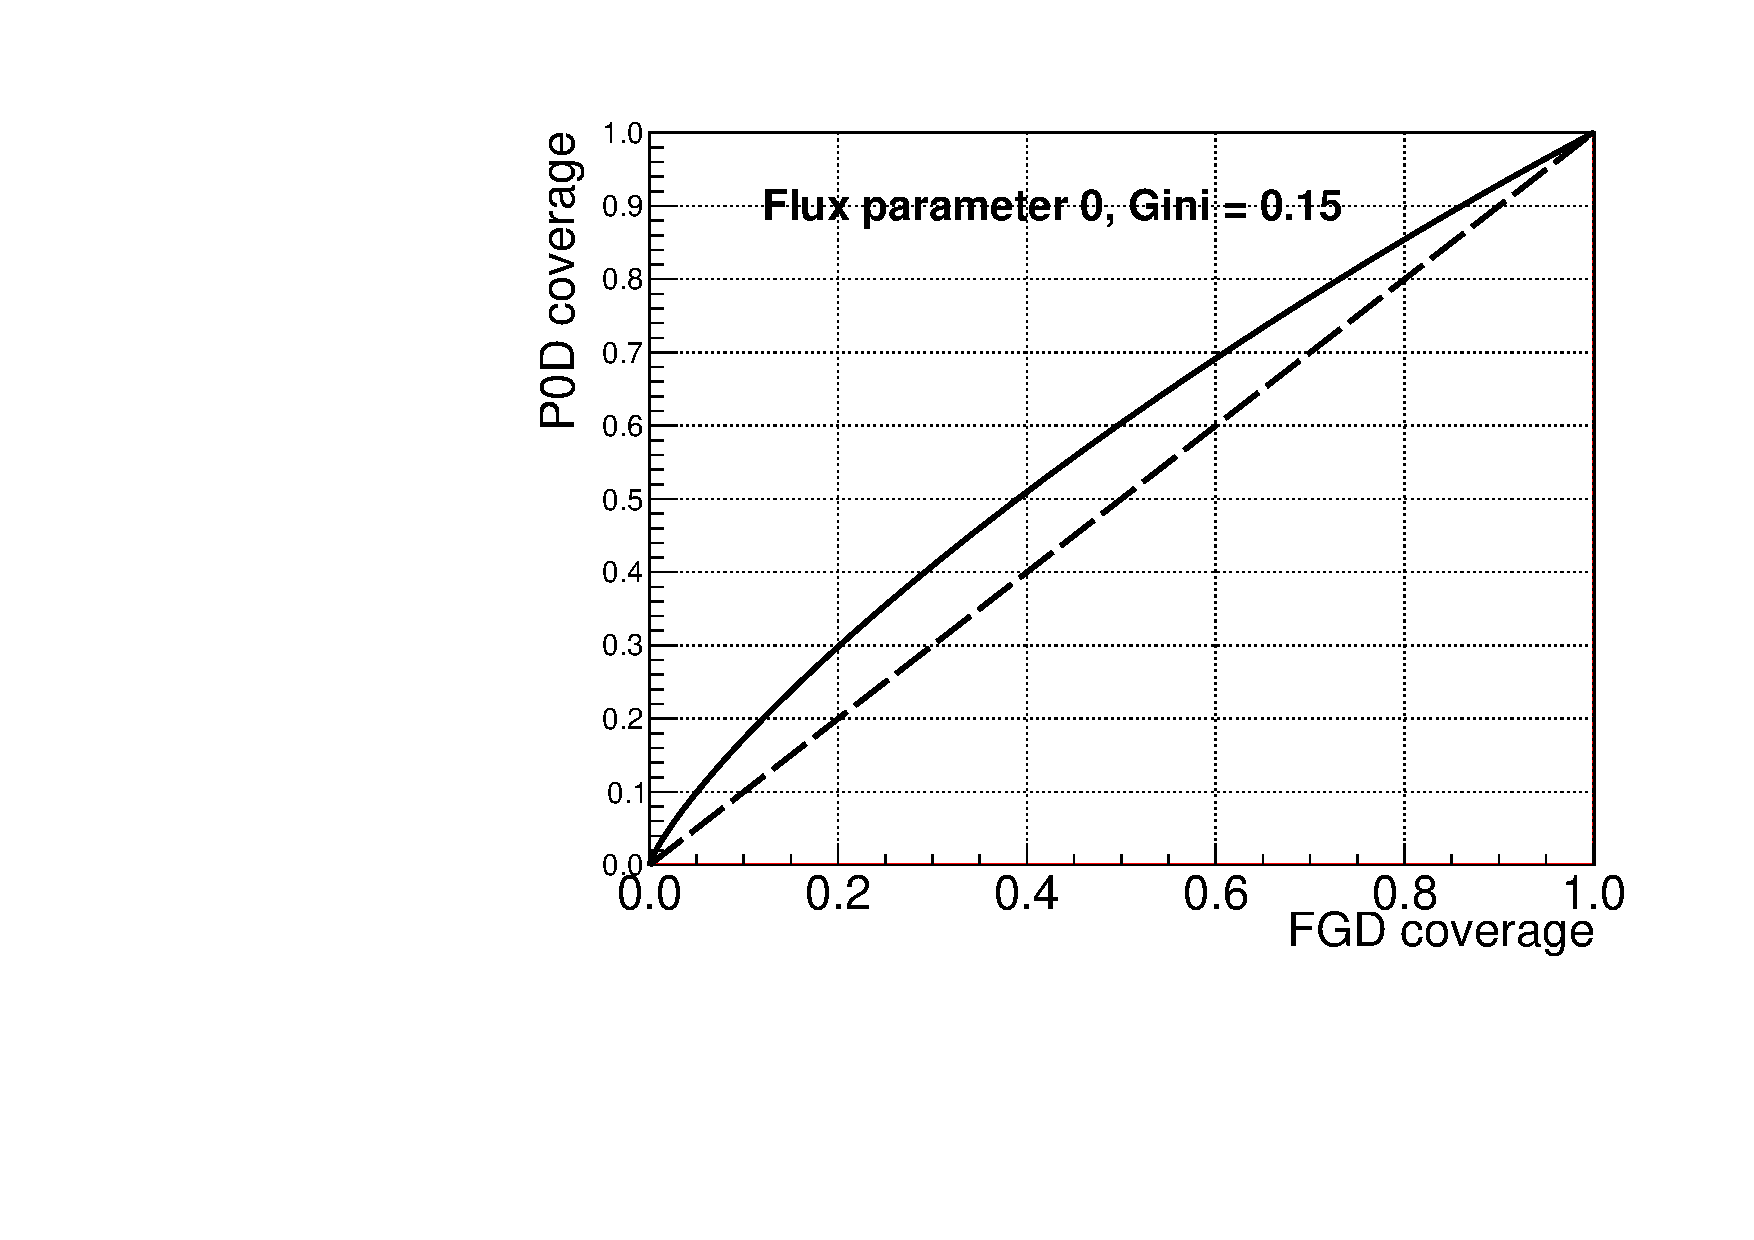
\includepdf[nup=3x5,pages={1-131},pagecommand=\thispagestyle{plain},width=2in]{/home/mhogan/Documents/graduateDisseration/Chapters/Figures/Discussion/ROC}
